\section{P-I-Kennlinie der Laserdiode}
\label{sect:durchführung}
Für die Vermessung der Laserdiode werden nur die beiden Linsen im Strahlengang justiert,
alle anderen Elemente sind entfernt.
Das Peltierelement wird auf 33.9$^\circ$C eingestellt und die Spannung an der
Photodiode bei verschiedenen Laserdiodenströmen aufgezeichnet.
\begin{figure}[H]
    \begin{center}
        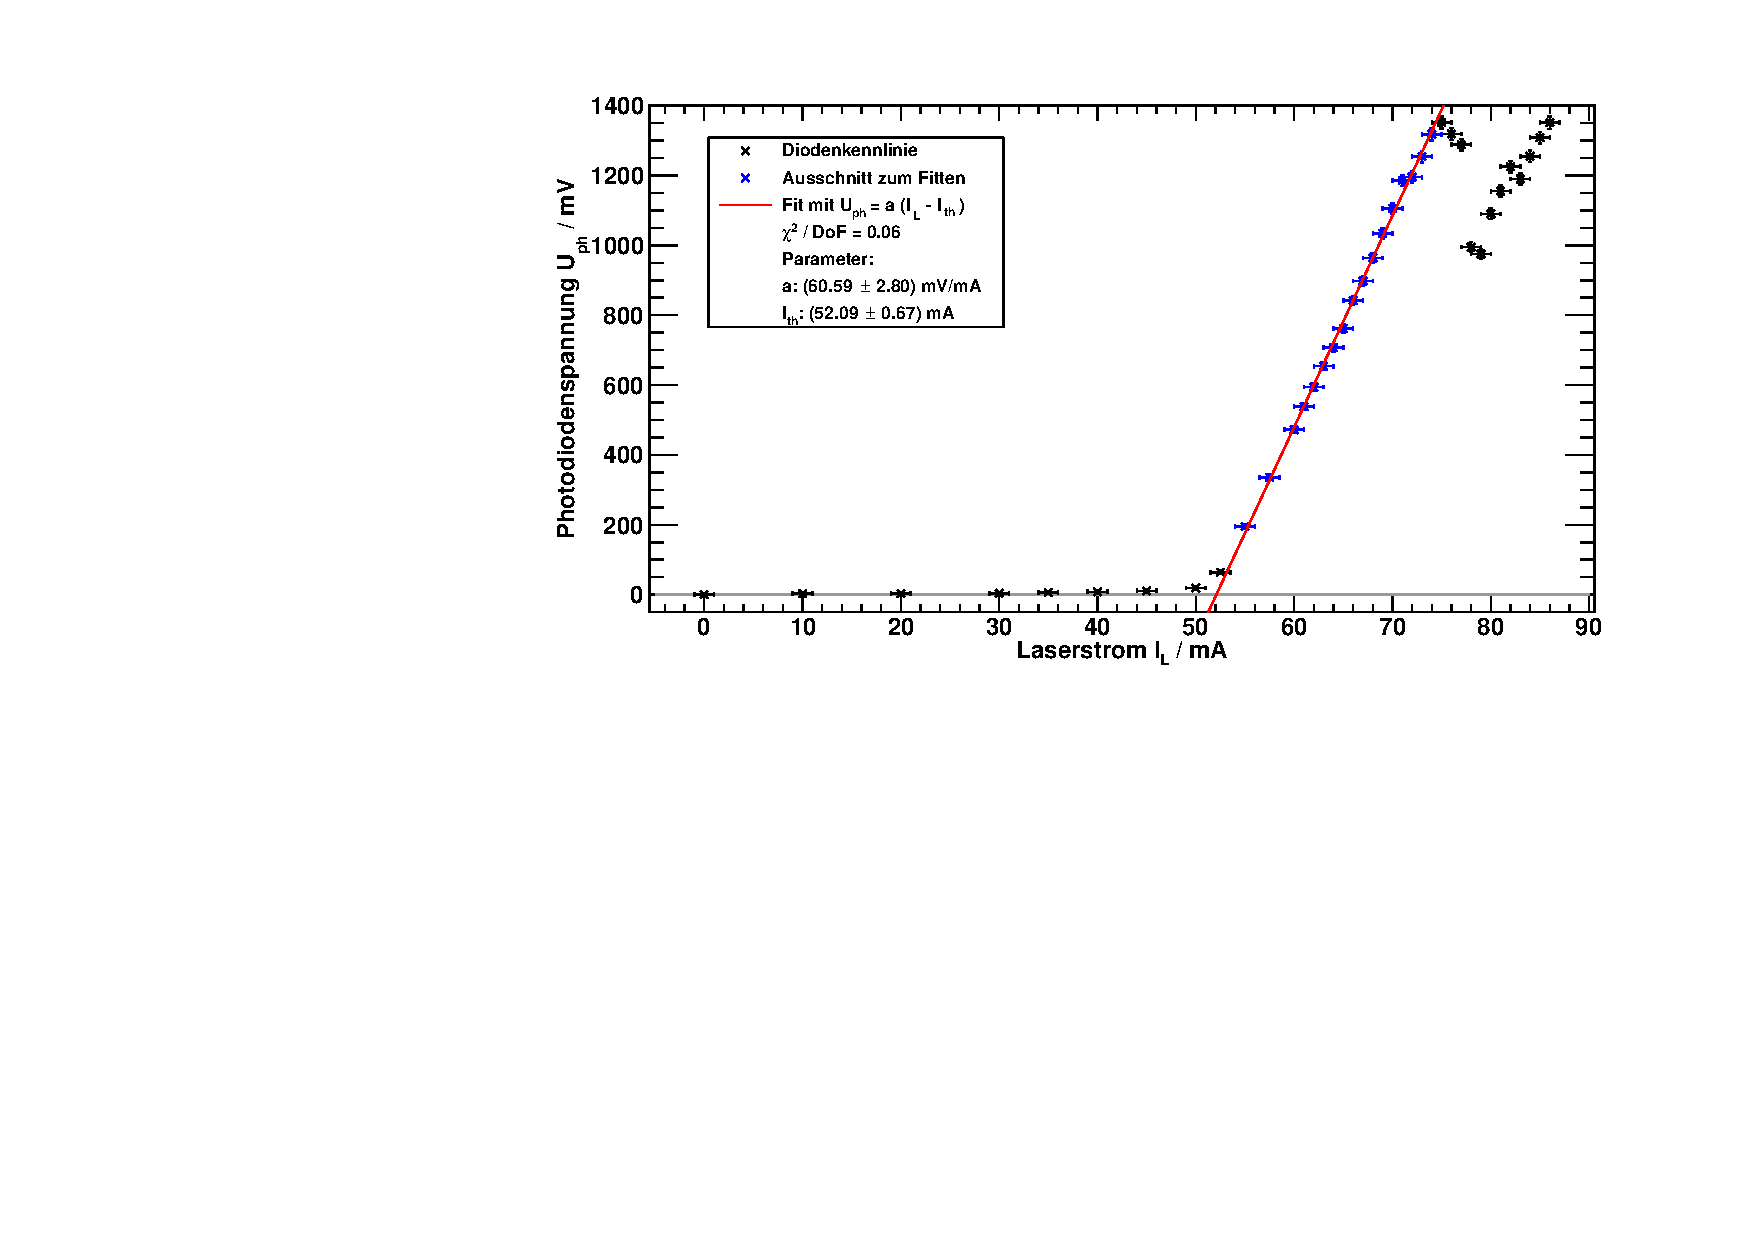
\includegraphics[width=\textwidth]{../img/part1/diodenkennlinie.pdf}
        \caption{$P$-$I$-Kennlinie der Laserdiode: Abhängigkeit der Spannung
        an der Photodiode vom Laserstrom $I_\text{L}$. Man erkennt den linearen Arbeitsbereich (gefitteter Teil),
        in dem ein modensprungfreier Betrieb möglich ist.}
        \label{img:Kennlinie}
    \end{center}
\end{figure}
\autoref{img:Kennlinie} zeigt die $P$-$I$-Kennlinie der Photodiode.
Als Fehler auf die Photodiodenspannung wurde ein Fehler von
\begin{equation}
    s_{U_{\text{ph}}}= 5\,\text{mV} + 0.01 \cdot U_{\text{ph}}
\end{equation}
angenommen.
Der Fehler auf den Strom $s_{I_{\text{L}}}$ beträgt ein Digit vom Lasernetzgerät:
\begin{equation}
    s_{I_{\text{L}}} = 0.1\,\text{mA} \ \, .
\end{equation}
Alle Messwerte wurden um den Spannungsoffset bei $I_{\text{L}}$=0\,mA verschoben.
Ein linearer Fit des modensprungfreien Laserbereichs zwischen 55\,mA und 71\,mA
liefert eine Laserschwelle $I_{\text{th}}$ von
\begin{equation}
    I_{\text{th}}=(52.01 \pm 0.13)\,\text{mA} \ \, .
\end{equation}
Interessant ist der Vergleich der $P$-$I$-Kennlinie mit dem Etalon-Transmissionsspektrum auf \autoref{img:etalon:fit}:
Aus der Amplitude der Modulationsspannung der Laserdiode und dem eingestellten Gleichanteil des Laserstroms
lässt sich der Laserstrom an den einzelnen Peaks bestimmen.
Dies wird hier kurz qualitativ gezeigt, ohne auf die Fehler einzugehen.

Der erste schwache Etalonpeak tritt bei einer Modulationsspannung von -0.26\,V auf, der Modensprung
bei einer Spannung von 0.22\,V.
Mit dem Konvertierungsfaktor des Lasernetzgeräts von 40\,mA/V und dem Gleichanteil des Laserstroms von 64.7\,mA
erhält man für den Laserstrom beim ersten Peak 54\,mA und beim Modensprung 74\,mA.
Dies entspricht fast exakt dem in der $P$-$I$-Kennlinie identifizierten Bereich
zwischen Laserschwelle und erstem Modensprung.



